
%%%%%%%%%%%%%%%%%%%%%%%%%%%%%%%%%%%%%%
\subsection{Installing Chisel on Ubuntu}
%%%%%%%%%%%%%%%%%%%%%%%%%%%%%%%%%%%%%%%

%*******************************************
\subsection{Scripts Directory}
%******************************************
If you are running Ubuntu, {\tt RTL/Scripts} contains useful installation scripts that automate the installation process.


%******************************************
\subsection{Install a Java Development Kit}
%*******************************************
Chisel is built on Scala, which requires the Java Development Kit (JDK). You have two options to install and manage the JDK.

%**************************************
\subsubsection{Install the Default JDK}
%**************************************        
\begin{bashcode}
sudo apt update && sudo apt install default-jdk
\end{bashcode}

%*********************
\subsubsection{SDKMan}
%*********************

SDKMAN! is a tool for managing parallel versions of Software Development Kits (SDKs) such as Java, Groovy, Kotlin, and more. It simplifies the installation, update, and switching between SDK versions.

\paragraph*{Installation}

To install SDKMAN!, open a terminal and run the following command:
\begin{bashcode}
     curl -s "https://get.sdkman.io" | bash       
\end{bashcode}

Add the following line to your .bashrc configuration file:
\begin{bashcode}
export SDKMAN_DIR="$HOME/.sdkman"
source "$SDKMAN_DIR/bin/sdkman-init.sh"
source ~/.bashrc
\end{bashcode}

After installation, restart your terminal or run:
\begin{bashcode}
    source "\$HOME/.sdkman/bin/sdkman-init.sh"        
\end{bashcode}

Verify the installation by running:
\begin{bashcode}
 sdk version    
\end{bashcode}       

\paragraph*{Using SDKMAN!}
Here are some common commands:

List All Available Java Versions:
\begin{bashcode}    
sdk list java
\end{bashcode}

Install a Specific Version
\begin{bashcode}
sdk install java 23-oracle   
\end{bashcode}

Set a Default Version
\begin{bashcode}
sdk default java 23-oracle    
\end{bashcode}

Switch Java Versions:
\begin{bashcode}
sdk use java 23-oracle    
\end{bashcode}

%******************************************
\subsection{Install Scala Build Tool (sbt)}
%******************************************
\begin{bashcode}
echo "deb https://repo.scala-sbt.org/scalasbt/debian all main" | \
sudo tee /etc/apt/sources.list.d/sbt.list && \
curl -sL "https://keyserver.ubuntu.com/pks/lookup? \ 
op=get&search=0x99E82A75642AC823" | \
sudo apt-key add && \
sudo apt update && \
sudo apt install sbt
\end{bashcode}


\paragraph{Clone this book}
Or use the template at 
\begin{bashcode}
https://github.com/chipsalliance/chisel
\end{bashcode}

\paragraph{Build and Run Your Chisel Project}
Navigate to your project's directory and use sbt to compile and run it:
\begin{bashcode}
cd your-chisel-project && sbt test
\end{bashcode}

%******************************
\subsection{Install Verilator}
%******************************
\begin{bashcode}
sudo apt-get install verilator
\end{bashcode}

For any operating system other than Ubuntu, see: https://verilator.org/guide/latest/install.html.

%******************************
\subsection{Install gtkwave}
%******************************
To view the waveforms created by verilator, instal gtkwave.
\begin{bashcode}
sudo apt-get install gtkwave
\end{bashcode}

%******************************
% \subsection{Install Vivado}
%******************************


%******************************
% \subsection{Install OpenLane}
%******************************

%******************************
% \subsection{Install OSS CAD Suite}
%******************************

%******************************
% \subsection{Install circt (firtool)}
%******************************

%%%%%%%%%%%%%%%%%%%%%%%%%%%%%
\subsection{Example Walkthrough}
%%%%%%%%%%%%%%%%%%%%%%%%%%%%%
Assuming you have cloned this book (Structured Computer Architecture), you will find the Chisel source files in the RTL/Chisel directory at the top level of the repository.

%***************************
\subsection{Key Directories}
%***************************
{\small
\begin{verbatim}
 RTL/Scripts:                              Installation scripts for Ubuntu 24.04
 RTL/Chisel/src/main/scala/scabook:        Chisel source files
 RTL/Chisel/test/scala/scabook:            Chisel test harness files
 RTL/Chisel/generated_verilog_clean:       SystemVerilog generated by Chisel 
 RTL/Chisel/generated_verlilog_annotated:  SystemVerilog with debug symbols
 RTL/Chisel/verilog_testbench:             Verilator C++ testbench files
\end{verbatim}
}

%***************************
\subsection{Run Chisel Test}
%***************************
The following very simple design generates a waveform
\includechiselcode[caption={Waveform Generator Code (Chisel)}, label={lst:chisel_waveformgenerator2}]{\chiselSourceDir/waveFormGenerator.scala}

The testbench for the code is:
\includechiselcode[caption={Waveform Generator Testbench Code (Chisel)}, label={lst:chisel_waveformgeneratortestbench}]{\chiselTestBenchSourceDir/waveFormGeneratorSpec.scala}

%*****************************
\subsection{Run the Testbench}
%*****************************
If you have cloned the textbook, build.sbt will be in your Chisel/ directory.
\includechiselcode[caption={Waveform Generator Testbench Code (Chisel)}, label={lst:build_sbt}]{RTL/Chisel/build.sbt}

The following commands will run the test bench
\begin{bashcode}
cd RTL/Chisel/
sbt test
\end{bashcode}

The IDE being used is Visual Studio Code with the Scala(Metals) extension installed. Your output should look something like:
\begin{bashcode}
(base) jglossner@jglossner-Alienware-Aurora-R7:~/GitRepos/Structured_Computer_Architecture/Chisel\$ sbt test
downloading sbt launcher 1.10.6
[info] welcome to sbt 1.10.5 (Oracle Corporation Java 23)
[info] loading settings for project chisel-build-build from metals.sbt ...
[info] loading project definition from /home/jglossner/GitRepos/Structured_Computer_Architecture/Chisel/project/project
[info] loading settings for project chisel-build from metals.sbt ...
[info] loading project definition from /home/jglossner/GitRepos/Structured_Computer_Architecture/Chisel/project
[success] Generated .bloop/chisel-build.json
[success] Total time: 1 s, completed Nov 30, 2024, 11:12:37 AM
[info] loading settings for project root from build.sbt ...
[info] set current project to %NAME% (in build file:/home/jglossner/GitRepos/Structured_Computer_Architecture/Chisel/)
[info] WaveFormGeneratorSpec:
[info] - WaveFormGenerator should generate the correct waveforms
[info] GCDSpec:
[info] - Gcd should calculate proper greatest common denominator
[info] Run completed in 8 seconds, 403 milliseconds.
[info] Total number of tests run: 2
[info] Suites: completed 2, aborted 0
[info] Tests: succeeded 2, failed 0, canceled 0, ignored 0, pending 0
[info] All tests passed.
[success] Total time: 9 s, completed Nov 30, 2024, 11:12:46 AM
\end{bashcode}

%*****************************************
\subsection{Generate Clean System Verilog}
%*****************************************
The only difference between the clean SystemVerilog and the annotated version is the commented out code.

For clean SystemVerilog:
\begin{chiselcode}
object WaveFormGenerator extends App {
  ChiselStage.emitSystemVerilogFile(
    new WaveFormGenerator,
    //Array("--target-dir", "generated")
    firtoolOpts = Array("-disable-all-randomization", "-strip-debug-info"),
  )
}
\end{chiselcode}

Run the SystemVerilog generator from the Chisel/ directory
\begin{bashcode}
sbt run
\end{bashcode}

This will produce
\includeverilogcode[caption={Clean SystemVerilog Code Produced by Chisel}, label={lst:chisel_waveformgeneratorcleanverilog}]{\verilogGeneratedByChiselSourceDir/WaveFormGenerator.v}

%***************************************************
\subsection{Generate Annotated/Debug System Verilog}
%***************************************************
This code will put the SystemVerilog simulation code directly into a generated folder
\begin{chiselcode}
object WaveFormGenerator extends App {
  ChiselStage.emitSystemVerilogFile(
    new WaveFormGenerator,
    Array("--target-dir", "generated")
    //firtoolOpts = Array("-disable-all-randomization", "-strip-debug-info"),
  )
}
\end{chiselcode}

The annotated/debug SystemVerilog generated code should look like:
\includeverilogcode[caption={Annotated SystemVerilog Code Produced by Chisel}, label={lst:chisel_waveformgeneratorannotatedverilog}]{RTL/Chisel/generators/generated/systemverilog_annotated/WaveFormGenerator.v}

%***********************************************
\subsection{Verilator C++ Test Driver} \label{sub:verilator_test_driver}
%***********************************************
Create a Verilator C++ test driver. It is in Chisel/verilator\_testbench
\includecppcode[caption={Verilator Testbench for WaveFormGenerator}, label={lst:verilator_waveformgenerator_testbench}]{\verilatorSourceDir/WaveFormGenerator_testbench.cpp}

From the RTL/Chisel/generators directory, execute:
\begin{bashcode}
verilator --cc ../generated_verilog_annotated/WaveFormGenerator.sv \
  --exe ../../verilator_testbench/WaveFormGenerator_testbench.cpp \
  --trace --Mdir obj_dir

make -C obj_dir -f VWaveFormGenerator.mk VWaveFormGenerator
\end{bashcode}

This will output the executable in Chisel/verilator\_testbench/obj\_dir

Execute the WaveFormGenerator program create in the obj\_dir
\begin{bashcode}
obj_dir/VWaveFormGenerator
\end{bashcode}

This will create a vcd file that can be displayed with gtkwave
\begin{bashcode}
gtkwave waveform.vcd    
\end{bashcode}

\begin{figure}[H]
    \centering
    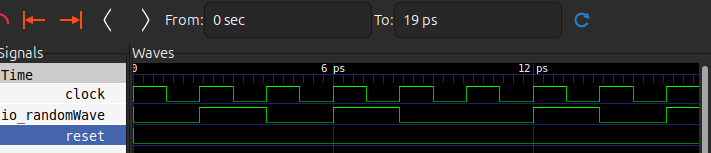
\includegraphics[width=\textwidth]{Images/verilator_waveformgenerator_screenshot.png} 
    \caption{Waveforms generated for a Verilator SystemVerilog simulation}
    \label{fig:verilator_wave2}
\end{figure}

%%%%%%%%%%%%%%%%%%%%%%%%%%%0
\subsection{Vivado Execution}
%%%%%%%%%%%%%%%%%%%%%%%%%%%%
Vivado is a comprehensive FPGA design suite developed by Xilinx. It integrates various tools for hardware design, simulation, synthesis, implementation, and debugging. Vivado supports Verilog, SystemVerilog, and VHDL for both design and simulation.

%**********************************
\subsection{Steps to Use Vivado}
%**********************************
\begin{enumerate}
    \item \textbf{Create a Project:}
    \begin{itemize}
        \item Open Vivado and create a new project.
        \item Specify the project type (RTL or post-synthesis).
        \item Add source files (e.g., Verilog, SystemVerilog, or VHDL).
    \end{itemize}

    \item \textbf{Write or Import a Testbench:}
    \begin{itemize}
        \item Add a testbench to simulate your design.
        \item Set the testbench as the top module for simulation.
    \end{itemize}

    \item \textbf{Simulate the Design:}
    \begin{itemize}
        \item Use the Vivado simulator to run behavioral simulations.
        \item Analyze the results in the waveform viewer.
    \end{itemize}

    \item \textbf{Synthesize and Implement:}
    \begin{itemize}
        \item Perform synthesis to generate a netlist.
        \item Run implementation to map the design to the FPGA.
    \end{itemize}

    \item \textbf{Generate a Bitstream:}
    \begin{itemize}
        \item Create a bitstream file to program the FPGA.
    \end{itemize}
\end{enumerate}

%************************************
\subsection{Key Features of Vivado}
%************************************
\begin{itemize}
    \item Supports advanced FPGA features such as high-speed transceivers and DSP blocks.
    \item Built-in waveform viewer for debugging simulations.
    \item Comprehensive support for Xilinx devices.
\end{itemize}

%********************************************
\subsection{Comparison of Vivado and Verilator}
%********************************************
Vivado and Verilator are both widely used in hardware design, but they cater to different needs. Below is a detailed comparison:

\begin{table}[htbp]
\renewcommand{\arraystretch}{2} % Adjust the row height (1.5x default)
\centering
\begin{tabular}{@{}p{4cm}p{5cm}p{4cm}@{}}
\toprule
\textbf{Feature}              & \textbf{Vivado}                                & \textbf{Verilator}                              \\ \midrule
\textbf{Purpose}              & Comprehensive FPGA design suite                & High-speed cycle-accurate simulation tool       \\
\textbf{Languages Supported}  & Verilog, SystemVerilog, VHDL                   & Verilog, SystemVerilog                         \\
\textbf{Test Driver Language} & HDL (Verilog/SystemVerilog/VHDL)               & C++ (or SystemC for advanced simulations)      \\
\textbf{Simulation Speed}     & Moderate (event-driven simulator)              & Very high (compiled C++ simulation)            \\
\textbf{Waveform Viewer}      & Built-in (integrated with simulation)          & Requires external tools like GTKWave (VCD)     \\
\textbf{FPGA Synthesis}       & Yes                                           & No                                             \\
\textbf{FPGA Targeting}       & Xilinx FPGAs                                   & Not applicable                                 \\
\textbf{Debugging Features}   & Integrated debugging and timing analysis tools & Debugging through C++ or external tools        \\
\textbf{Open Source}          & No (proprietary software)                      & Yes (GPL-licensed)                             \\ \bottomrule
\end{tabular}
\caption{Comparison of Vivado and Verilator}
\label{tab:vivado_vs_verilator}
\end{table}

\subsection*{When to Use Vivado vs. Verilator}

\begin{itemize}
    \item \textbf{Use Vivado:}
    \begin{itemize}
        \item When designing and implementing FPGA designs targeting Xilinx devices.
        \item If you require a complete toolchain for synthesis, implementation, and simulation.
        \item For designs involving VHDL.
    \end{itemize}
    \item \textbf{Use Verilator:}
    \begin{itemize}
        \item For high-speed simulations of Verilog/SystemVerilog designs.
        \item When testing large designs with long simulation runs.
        \item For open-source or academic projects where licensing costs are a concern.
    \end{itemize}
\end{itemize}



The following is the SystemVerilog module `waveFormGenerator`, which generates a random waveform and a clock signal:

\includeverilogcode{RTL/Verilog/src/WaveFormGenerator.sv}


\subsection*{SystemVerilog Testbench}

The testbench for the `waveFormGenerator` module monitors its signals during simulation:

\begin{verilogcode}[caption={SystemVerilog Testbench for waveFormGenerator}]
`timescale 1ns/1ps

module waveFormGenerator_tb;
    logic randomWave;
    logic clock;

    // Instantiate the DUT (Device Under Test)
    waveFormGenerator dut();

    initial begin
        $monitor("Time: %0t | randomWave: %b | clock: %b", $time, dut.randomWave, dut.clock);
        #30 $finish; // End the simulation after 30 time units
    end
endmodule
\end{verilogcode}

\subsection*{Explanation}

\subsection*{Module Details}
The `waveFormGenerator` module generates:
\begin{itemize}
    \item A `randomWave` signal with values that change at specified time delays.
    \item A `clock` signal that toggles every 2 time units.
\end{itemize}

\subsection*{Testbench Details}
The testbench:
\begin{itemize}
    \item Instantiates the `waveFormGenerator` module.
    \item Monitors the `randomWave` and `clock` signals using `\$monitor`.
    \item Ends the simulation after 30 time units with `\$finish`.
\end{itemize}